\chapter{Edge Detection Using OpenCV} \label{chap:Edge Detection Using OpenCV}

The internship project began with the final objective of automating the \ac{AR} camera lens calibration. For that, the following tasks were outlined:
\begin{enumerate}
    \item Develop a program that detects the coordinates (in pixels) of the corners of a quadrilateral target, as well as the corresponding centroid.
    \item Using the centroid coordinates, calibrate the central-shift.
    \item Using the coordinates of the corners of the target, calibrate the FoV and \( k_1 \)/\( k_2 \) coefficients.
    \item Calibrate the nodal point.
\end{enumerate}

The objective is to recreate the calibration procedure that an operator uses. The following sections explain in detail how each task is completed, as well as the limitations and advantages of the current methods.



\section{Canny Edge Detection}
Even though OpenCV cannot directly provide the coefficients required, this library still proves useful for its powerful image object detection functions. 

\noindent Canny edge detection is a multi-step algorithm designed to detect a wide range of edges in images. It begins with noise reduction—typically using a Gaussian filter—to smooth the image and minimize the impact of noise. Next, the algorithm computes the intensity gradients to identify areas with rapid intensity changes, which serve as potential edge locations. To refine these candidate edges, non-maximum suppression is applied to thin the detected edges, ensuring that only the strongest responses are retained. Finally, double thresholding and edge tracking by hysteresis are used to classify edges as strong or weak, and to connect weak edges that are likely part of the same boundary structure \cite{opencv_canny, geeksforgeeks_canny}. An example of Canny's capabilities is shown in figure \ref{fig:pumpkin}.
\begin{figure}[h]
    \centering
    \includegraphics[width=\textwidth]{Images/03edgedetect/pumpkin.png}
    \caption{Example of a canny edge detection application \cite{geeksforgeeks_canny}}
    \label{fig:pumpkin}
\end{figure}


\noindent In the context of this project, the Canny edge detection algorithm is employed to automatically identify the boundaries of a quadrilateral target by using the OpenCV contour approximation functions \cite{contour_approximation, contour}. By accurately detecting the corners and the centroid of the target, the algorithm provides the critical coordinates necessary for calibrating the AR camera lens. These coordinates form the basis for subsequent calibration steps such as central-shift correction, Field of View (FoV) adjustments, and compensation for lens distortion coefficients. The robustness of the Canny method against varying lighting conditions and noise makes it particularly effective for this application.

\noindent For more detailed explanations on the workings and implementation of the Canny edge detection algorithm in Python using OpenCV, readers are encouraged to consult the OpenCV tutorial \cite{opencv_canny} and the GeeksforGeeks guide \cite{geeksforgeeks_canny}. These resources provide insights into the algorithm's multi-stage process and practical considerations in real-world applications.

\noindent The edge detection capabilities of OpenCV were used to 
provide the results shown in Figure \ref{fig:corners}.

\begin{figure}[h]
    \centering
    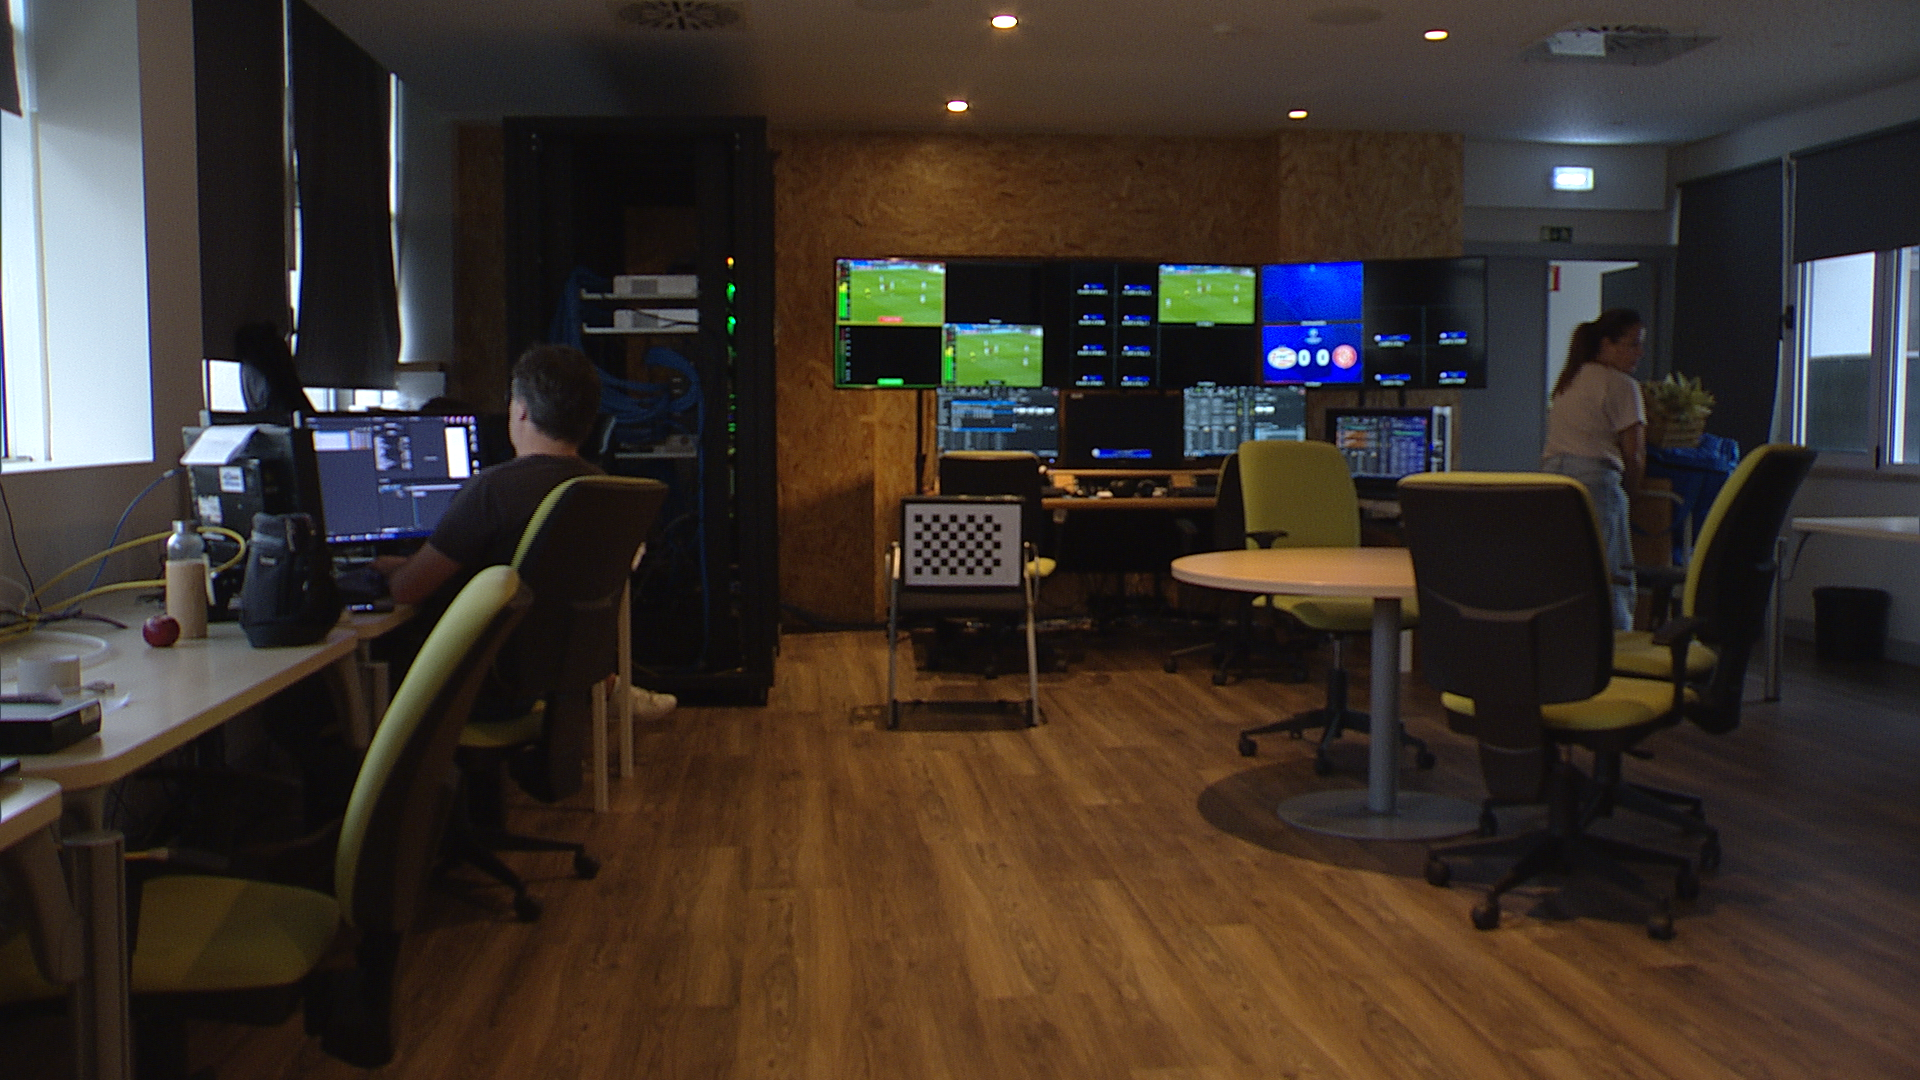
\includegraphics[width=\textwidth]{Images/02stateart/br1.png}
    \caption{Image taken with the camera with the target at the center}
    \label{fig:target}
\end{figure}

\begin{figure}[h]
    \centering
    \includegraphics[width=\textwidth]{Images/02stateart/edge_detection.png}
    \caption{Edge detection program demonstration}
    \label{fig:corners}
\end{figure}

\noindent This program enables the detection of the coordinates of the corners and the center of the target, as well as determining the length and width dimensions of the target.

\noindent In conclusion, this section has described the role of Canny edge 
detection in the project, 
emphasizing its utility in identifying the quadrilateral target's corners and centroid. 
The effective detection of these key points supports the calibration process, leading to 
more accurate adjustments in central-shift, FoV, and lens distortion parameters.

\section{Using Blender for Testing}
\label{sec:blender_workflow}
\noindent To evaluate the effectiveness of this program, multiple images from different angles and levels of distortion were needed. However, since the camera is not always available for this project, another program called "Blender" was used to simulate images that would resemble those provided by the real camera. Blender is a free and open-source 3D computer graphics software widely used for creating 3D models, animations, visual effects, and more. In this case, Blender was used to create a virtual camera and virtual targets.

\noindent This section outlines the workflow for setting up and rendering a scene in Blender, a widely used open-source 3D modeling and animation software. The following steps detail how to navigate the interface, adjust objects and camera settings, and produce a rendered image, as applied in this study. Blender was used in this project for simulating images for testing.

\begin{enumerate}
    \item \textbf{Loading a Scene}: Launch Blender and load the desired scene file to begin working with the 3D environment like in figure \ref{fig:load}.
    \begin{figure}[h]
        \centering
        \includegraphics[width=\textwidth]{Images/03edgedetect/1.png}
        \caption{Loading a Scene}
        \label{fig:load}
    \end{figure}

    \item \textbf{Viewport Navigation}: To explore the scene in the Viewport:
    \begin{itemize}
        \item Drag the middle mouse button (MMB) to rotate the view.
        \item Hold Shift and drag MMB to pan across the scene.
        \item Use the mouse wheel to zoom in or out.
    \end{itemize}
    
    \item \textbf{Adjusting Object Positions}: Select the target object (e.g., \texttt{Target\_1} or \texttt{Target\_2}) from the right-hand menu. Modify its position and orientation by:
    \begin{itemize}
        \item Dragging the left mouse button (LMB) on the \textit{Location} and \textit{Rotation} fields.
        \item Typing specific values directly.
        \item Using the interface arrows for incremental adjustments.
    \end{itemize}

    Figure \ref{fig:adjust} illustrates this procedure.

    \begin{figure}[h]
        \centering
        \includegraphics[width=\textwidth]{Images/03edgedetect/2.png}
        \caption{Adjusting Object Positions}
        \label{fig:adjust}
    \end{figure}

    \item \textbf{Aligning the Viewport to the Camera}: To preview the camera’s perspective, press \texttt{Numpad-0} (the zero key on the numeric keypad).
    
    \item \textbf{Camera Positioning}: Select the \texttt{CAMERA\_MANIPULATOR} object and adjust its \textit{Location} and \textit{Rotation} parameters, following the same method as for target objects.
    \begin{figure}[h]
        \centering
        \includegraphics[width=\textwidth]{Images/03edgedetect/3.png}
        \caption{Camera Positioning}
    \end{figure}
    \item \textbf{Camera Lens Settings}: Select the child object \texttt{Camera} under \texttt{CAMERA\_MANIPULATOR}, then access the \textit{Data} sub-menu (indicated by a green camera icon in the bottom-right panel), figure \ref{fig:setting}. Adjust the following:
    \begin{itemize}
        \item \textit{Shift X / Shift Y}: Modify the center shift in the X and Y directions.
        \item \textit{Focus Distance}: Set the camera’s focus point.
        \item \textit{F-Stop}: Control depth of field; lower values increase blur for objects outside the focus distance, while higher values extend the in-focus range.
        \item \textit{Focal Length}: Adjust this parameter (bottom-left corner) to change the field of view (FoV), reflected on the right-hand side.
        \item \textit{K1 and K2}: Edit distortion coefficients directly below the \textit{Focal Length}.
        \item \textit{Nodal Offset}: Represented by the Y-value in the \textit{Location} parameter (displayed in purple). Right-click and select \textit{Edit Driver} to modify its governing function.
    \end{itemize}
    \begin{figure}[h]
        \centering
        \includegraphics[width=\textwidth]{Images/03edgedetect/4.png}
        \caption{Camera Lens Settings}
        \label{fig:setting}
    \end{figure}
    \item \textbf{Rendering the Image}: From the top-left menu, select \textit{Render $\rightarrow$ Render Image} to initiate the rendering process, figure \ref{fig:render}.
    \begin{figure}[h]
        \centering
        \includegraphics[width=\textwidth]{Images/03edgedetect/5.png}
        \caption{Rendering the Image}
        \label{fig:render}
    \end{figure}
    \item \textbf{Saving the Render}: In the rendering window, wait for the sample calculations to complete, then choose \textit{Image $\rightarrow$ Save As...} to save the output, figure \ref{fig:save}.
    \begin{figure}[h]
        \centering
        \includegraphics[width=\textwidth]{Images/03edgedetect/6.png}
        \caption{Saving the Render}
        \label{fig:save}
    \end{figure}
    
    \item \textbf{Data Collection}: Currently, data extraction from the rendered image is performed manually. Automation of this process is feasible and could be implemented if deemed beneficial for future work.
\end{enumerate}

\noindent This workflow demonstrates Blender’s capability for precise scene manipulation and rendering, making it a valuable tool for 3D visualization in this research.
To test the edge detection program, only one target was used. Multiple pictures from different angles and with varying distortions were taken and tested. Some of the results are shown in Figure \ref{fig:Edge Detection Results Visualization}.

\begin{figure}[h!]
    \centering
    % First row
    \begin{subfigure}[b]{0.45\textwidth}
        \centering
        \includegraphics[width=\textwidth]{Images/02stateart/edge_detection_1.png}
        \caption{Image 1}
    \end{subfigure}
    \hfill
    \begin{subfigure}[b]{0.45\textwidth}
        \centering
        \includegraphics[width=\textwidth]{Images/02stateart/edge_detection_2.png}
        \caption{Image 2}
    \end{subfigure}
    
    \vspace{1cm}
    
    % Second row
    \begin{subfigure}[b]{0.45\textwidth}
        \centering
        \includegraphics[width=\textwidth]{Images/02stateart/edge_detection_3.png}
        \caption{Image 3}
    \end{subfigure}
    \hfill
    \begin{subfigure}[b]{0.45\textwidth}
        \centering
        \includegraphics[width=\textwidth]{Images/02stateart/edge_detection_4.png}
        \caption{Image 4}
    \end{subfigure}
    
    \vspace{1cm}
    
    % Third row
    \begin{subfigure}[b]{0.45\textwidth}
        \centering
        \includegraphics[width=\textwidth]{Images/02stateart/edge_detection_5.png}
        \caption{Image 5}
    \end{subfigure}
    \hfill
    \begin{subfigure}[b]{0.45\textwidth}
        \centering
        \includegraphics[width=\textwidth]{Images/02stateart/edge_detection_6.png}
        \caption{Image 6}
    \end{subfigure}
    
    \vspace{1cm}
    
    % Fourth row
    \begin{subfigure}[b]{0.45\textwidth}
        \centering
        \includegraphics[width=\textwidth]{Images/02stateart/edge_detection_7.png}
        \caption{Image 7}
    \end{subfigure}
    \hfill
    \begin{subfigure}[b]{0.45\textwidth}
        \centering
        \includegraphics[width=\textwidth]{Images/02stateart/edge_detection_8.png}
        \caption{Image 8}
    \end{subfigure}
    
    \caption{Edge Detection Results Visualization}
    \label{fig:Edge Detection Results Visualization}
\end{figure}

\noindent From these tests, we can confirm that the program works as intended. Even for distorted images.

\noindent This method, however, presents certain limitations. When tested in real-world scenarios, the program occasionally misidentified the real target due to interference from ambient lighting. To mitigate this issue, the target color was changed from white to red, as red is a less common color in real-world environments and contrasts well in studio settings that employ green screens.